

\chapter[Nondipole effects in HHG using noncollinear bicircular beams]{Nondipole effects in high-order harmonic generation using noncollinear bicircular beams}
%\chaptermark{Nondipole effects in HHG using noncollinear bicircular beams}
\label{chap:nondipole-HHG}
In this chapter we turn to the extension of HHG in another frontier -- the extension of the plateau to higher harmonic cutoffs, in the search for shorter wavelengths and the possibility of shorter pulses and experiments at higher temporal resolutions. 

At first brush, increasing the HHG cutoff -- $\Omega_\mathrm{max}=I_p + 3.17U_p$ -- is simply a technological challenge in increasing the intensity and using longer wavelengths, and ensuring that the phase matching works. However, there is also a fundamental limit, because as the cutoff energy increases, the electron will eventually be fast enough that the Lorentz force, $\vbf_\mathrm{m}=\vbv/c\times\vbb$, becomes significant.

In this chapter we develop and test a way to overcome this limitation, by using building of the constructions of the chapter~\ref{chap:spin-HHG}: the use of two counter-rotating circularly polarized driving lasers, this time at equal frequencies and with non-collinear propagation directions.




The material in this chapter has previously appeared in reference

\begin{enumerate}
\item[{\hypersetup{citecolor=black}\citealp{Pisanty_lorentz_2016}}.]
\textsc{E.~Pisanty, D.~D. Hickstein, B.~R. Galloway, C.~G. Durfee, H.~C. Kap\-teyn, M.~M. Murnane and M.~Ivanov}.
\newblock High harmonic interferometry of the Lorentz force in strong
  mid-infrared laser fields. \href{http://arxiv.org/abs/1606.01931}{arXiv:1606.01931} (2016).
\end{enumerate}


\noindent
Moreover, the extensions to the Lewenstein-model SFA calculations are implemented and openly available as

\begin{enumerate}
\item[{\hypersetup{citecolor=black}\citealp{RB-SFA}}.]
\textsc{E.~Pisanty}. RB-SFA: High Harmonic Generation in the Strong Field Approximation via Mathematica. \url{https://github.com/episanty/RB-SFA} (2016).
\end{enumerate}





\section{The Lorentz force in high-order harmonic generation}

As we saw in chapter~\ref{chap:HHG-intro}, high-order harmonic generation generally produces a flat plateau of harmonics that extends through to the high-harmonic cutoff at frequency
\begin{equation}
\Omega_\mathrm{max}=I_p + 3.17U_p = I_p + 3.17 \frac{F^2}{4\omega^2}.
\end{equation}
In general, one of the goals of the field is to extend this cutoff frequency, by using higher intensities and longer driving wavelengths, since higher cutoffs open new experimental regimes with bigger photon energies, such as exploration of the water window using bright and coherent soft x-ray microscopes, and the testing of ultrafast phenomena at even faster time-scales, such as relaxation phenomena in core electrons in biological molecules, among~others. 

To a certain extent -- or, at least, as far as the three-step model is concerned -- increases in the field intensity and wavelength are roughly equivalent, since they both increase $U_p$ and decrease the Keldysh parameter $\gamma$. However, there is a definite preference for increasing the cutoff via increases in the driver wavelength, since increasing the intensity too much will eventually saturate the ionization of the sample, and while one can hope for high-harmonic emission from highly charged ionic species, it has yet to be experimentally demonstrated.

Increasing the wavelength, on the other hand, increases the ponderomotive energy of the field (essentially, by giving the electron a longer time in which to harvest energy from the field), without risking ionization saturation. Producing high-intensity laser systems at wavelengths longer than $\SI{800}{nm}$ is a technological challenge, mostly met via optical parametric chirped-pulse amplifiers, and while longer wavelengths do offer lower intensities and repetition rates than the better tested titanium-sapphire technology, the available intensities at long wavelength are rising and are predicted to continue increasing as technology develops.

Beyond this technological limitation, long-wavelength HHG is limited by the fact that, with the electron spending longer times in the continuum, its wavepacket will spread further, which then diminishes the recollision probability. Moreover, as the driving wavelength increases and the harmonic wavelength becomes ever shorter, the challenges posed by phase matching can change considerably~\cite{popmintchev_phase-matching_2009}. Nevertheless, both of these limitations can be successfully addressed, and harmonics as high as $\SI{1.4}{keV}$ -- with harmonic orders as high as $5000$ -- have been produced using $\SI{3.9}{\micro m}$ drivers~\cite{ popmintchev_record_2012}. Indeed, wavelengths as high as $\SI{10.6}{\micro m}$ are under consideration~\cite{ hernandez_nine-micron_2013, zhu_non-dipole_2016, emelina_possibility_2014}.




However, this programme runs into a surprising limitation in that the dipole approximation breaks down in the \textit{long} wavelength regime: as the wavelength increases, the electron has progressively longer times to accelerate in the field, and the magnetic Lorentz force $\vbf_\mathrm{m}=\vbv/c \times \vbb$ becomes significant~\cite{reiss_dipole-approximation_2000}. This pushes the electron along the laser propagation direction and, when strong enough, makes the electron wavepacket completely miss its parent ion, quenching all recollision phenomena, including high harmonic generation~\cite{potvliege_photon_2000, walser_hhg_2000,kylstra_photon_2001, kylstra_photon_2002, chirila_analysis_2004, chirila_nondipole_2002, milosevic_relativistic_2002, milosevic_relativistic_2002-1, emelina_possibility_2014} (but also extending e.g. to above-threshold ionization~\cite{klaiber_above-threshold_2005}). In this regime, the usual harmonic plateau drops by several orders of magnitude and it loses intensity at the cutoff, as showcased in \reffig{f6-emelina-original-spectrum}.


Multiple schemes have been proposed to overcome this limitation, falling along two main lines: the generating medium, and the driving fields. On the side of the medium, proposals have ranged from 
%
antisymmetric molecular orbitals~\cite{ fischer_enhanced_2006} 
%
through relativistic beams of highly-charged ions~\cite{ mocken_bound-mev_2004, avetissian_high-order_2011}
% 
to exotic matter like positronium~\cite{henrich_positronium_2004, hatsagortsyan_microscopic_2006} 
%
or muonic atoms~\cite{muller_exotic_2009}. 
%
Most of these represent significant challenges in target engineering, and the only one that is currently feasible, the use of antisymmetric molecular orbitals to ionize from one site and recombine on the other, has limited ability in terms of the Lorentz drift it can accommodate.



\begin{figure}[t!]
  \centering
  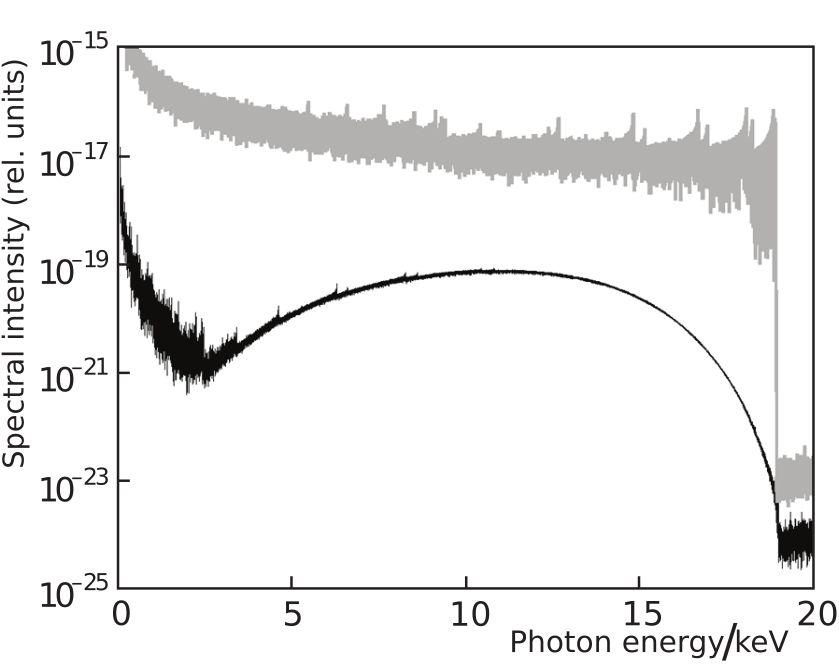
\includegraphics[scale=1.15]{9-Nondipole-HHG/Figures/figure9A.png}
  \caption[
  Damping of HHG emission by the Lorentz force at $\SI{8}{\micro\meter}$ and $\SI{e15}{W/cm^2}$, by several orders of magnitude with respect to the dipole-approximation ideal, as calculated by A.S. Emelina~et~al.
  ]{
  Damping by the Lorentz force of the harmonic emission of helium under a six-cycle pulse at $\SI{8}{\micro\meter}$ and $\SI{e15}{W/cm^2}$, as compared to the same conditions under the dipole approximation, shown in gray.
  Figure excerpted from \citer{emelina_possibility_2014}.
  }
\label{f6-emelina-original-spectrum}
\end{figure}
\copyrightfootnote{
\reffig{f6-emelina-original-spectrum} © IOP Publishing. Reproduced with permission. All rights reserved.
}
%% Copyright note is temporary pending IOP reply.




Similarly, driving-field proposals also represent significant challenges. The proposed methods include 
%
counter-propagating mid-IR beams~\cite{ taranukhin_relativistic_2000, taranukhin_high-order_2002, milosevic_lasers-attosecond-nuclear_2004, verschl_relativistic_2007,verschl_consecutive-laser-pulses_2007}, 
%
the use of auxiliary fields propagating in orthogonal directions~\cite{ chirila_nondipole_2002}, 
%
fine tailoring of the driving pulses~\cite{klaiber_relativistic_2006, klaiber_fully_2007,liu_laser-guided_2009}, 
%
coun\-ter-propagating trains of attosecond pulses~\cite{ hatsagortsyan_laser_driven_2008, kohler_phase-matched_2011} 
in the presence of strong magnetic fields \cite{verschl_refocussed_2007}, 
%
and collinear and non-collinear X-ray initiated HHG~\cite{klaiber_coherent_2008, kohler_macroscopic_2012}. 
%
Generally, these methods also pose significant challenges: as examples, counter-propagating beams make it very hard to direct the harmonic emission into a single beam, orthogonal beams severely limit the interaction region, and finely-tailored pulses have yet to be demonstrated at sufficient intensity to produce harmonic emission. 

Perhaps most promisingly, it is possible to eliminate the effect of the magnetic force, at least in parts of the interaction region, with the use of a very tight focus for the driving laser~\cite{liu_laser-guided_2009, lin_tight-focus_2006}, which can also be extended to long-wavelength light in narrow waveguides~\cite{galloway_lorentz_2016}. This method uses the fact that, in a tight laser focus, scalar optics fails, and the vector optics of a gaussian focus give a field with a nonzero component along the propagation direction~\cite{maltsev_nondipole-ati_2003}, which can then be used to manipulate the continuum electron's motion along this direction. 

Unfortunately, this method requires a very tight focus to work; the required focal lengths are within the present possibilities, but this still presents severe challenges through its impact on phase matching. Moreover, the effect will vary, strongly, across the focus~\cite{galloway_lorentz_2016}, making the far-field properties of the emission a complete (but interesting) unknown at this point.






\section{Cancelling the Lorentz force with noncollinear beams}
In this chapter we will propose and develop an alternative method for dealing with the Lorentz force, which will allow experiments that cancel this drift to re-enable harmonic emission as well as to probe it and demonstrate it in HHG experiments using currently available technology.

We address the motion in the propagation dimension using a forwards-elliptical field~-- a field with a polarization ellipse with a minor axis along the propagation direction, or more specifically along the direction of the Lorentz force -- exactly as achieved by the tight-focussing scheme described above. However, there is a much simpler way to achieve this ellipticity, and it is through the use of two counter-rotating, bicircular fields, of the same frequency, which are focussed non-collinearly, as shown in \reffig{f8-field-configuration}.


\begin{figure}[htb]
  \centering
  \subfloat{\label{f8-field-configuration-beams}}
  \subfloat{\label{f8-field-configuration-ellipses}}
  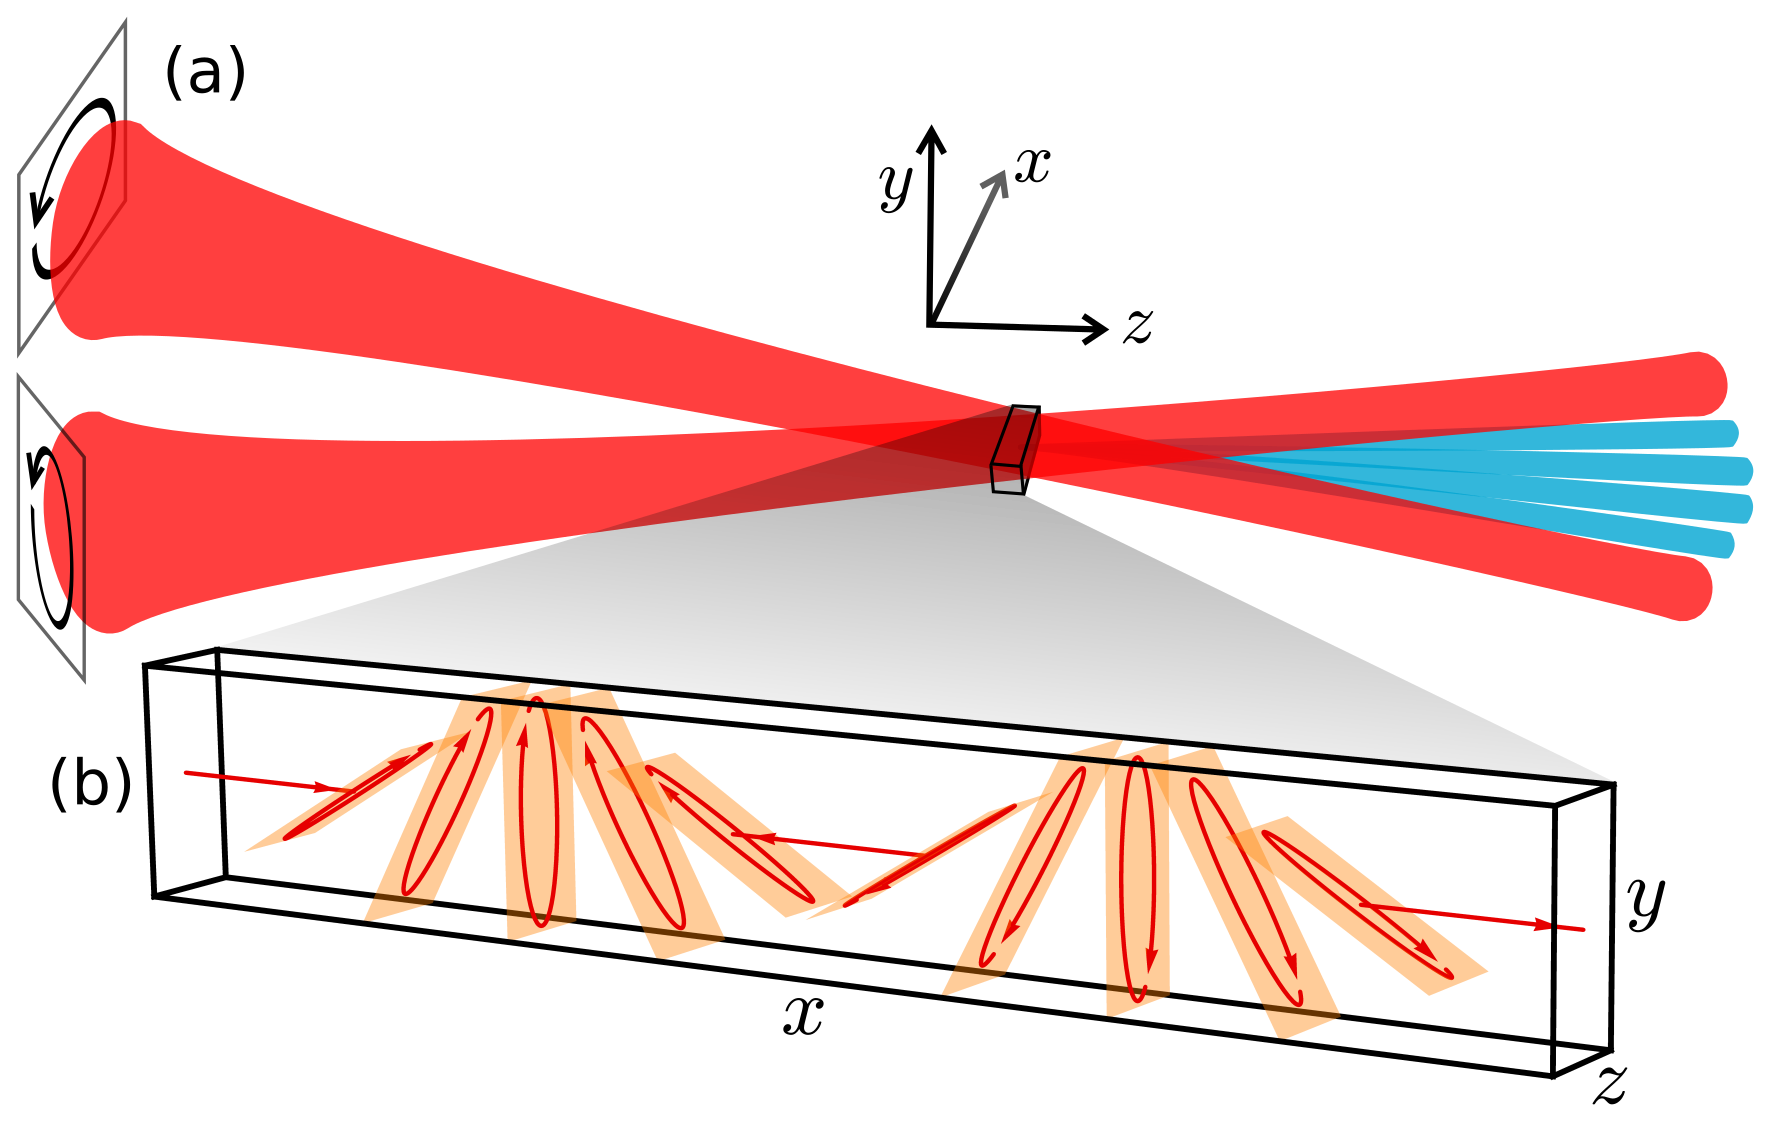
\includegraphics[width=0.7\textwidth]{9-Nondipole-HHG/Figures/figure9B.png} 
  \caption[
  Proposed beam configuration for probing the Lorentz-force action: two non-collinear, counter-rotating circularly polarized beams of the same frequency, with the resulting field configuration showing forwards ellipticity
  ]{
  The proposed beam configuration \protect\subref{f8-field-configuration-beams}, with two non-collinear, counter-rotating circularly polarized beams converging on a gas jet, typically at a beam half-angle $\theta$ of the order of \SI{5}{\degree}. At their focus, the two beams generate a polarization gradient~\protect\subref{f8-field-configuration-ellipses} which includes points with an elliptical polarization with the minor axis along the centreline of the system.
  }
\label{f8-field-configuration}
\end{figure}



In general, adding two coplanar circular polarizations at the same frequency simply results in a linear polarization at that frequency, with the polarization direction determined by the relative phase between the two circular components. Here, however, the two circular polarizations are \textit{not} coplanar, since the propagation directions are at a slight angle, which means that they have a nonzero component along the centreline of the system, the $z$ axis of \reffig{f8-field-configuration}, and this component of the two fields can still add constructively to give an elliptical polarization with the minor axis along the centreline. Conversely, at these points the off-plane magnetic field components of the two beams cancel out, giving a Lorentz force along the centreline and in the plane of ellipticity of the electric field.

This configuration, then, affords us a good measure of control over the propagation-direction component of the electric field, and therefore allows us to influence the motion of the electron in this direction. Most interestingly, the electric field component can be chosen to guide the electron back to the ion even in the presence of a nonzero Lorentz force.

However, this can only happen once per period, because the symmetries of the Lorentz force and the forwards ellipticity do not match: the Lorentz force pushes forward along the propagation direction on both half-cycles (as shown in \reffig{f8-schematic-trajectories-c}) and the ellipticity pushes backwards for one ionization burst but forwards on the other (as shown in \reffig{f8-schematic-trajectories-b}), so while one trajectory can be recovered, the other ionization burst will be inevitably lost. This will, of course, have an impact on the signal -- but half of the signal we initially wanted is still an improvement over no signal at all.




More importantly, however, this break in the symmetry between half-cycles also leaves clear marks on the spectrum, in particular through the presence of even harmonics. With a linear driving field (even in the presence of the magnetic Lorentz force), the contributions to the even harmonics of the two opposite recollisions in each laser cycle exactly cancel, leaving only the odd harmonics observed in \reffig{f7-standard-harmonic-spectrum}. Here, however, the two half cycles have different weight (and indeed one of them may not emit at all), so the result will be a signal in the even harmonics. 


\begin{figure}[t!]
  \centering
  \subfloat{\label{f8-schematic-trajectories-a}}
  \subfloat{\label{f8-schematic-trajectories-b}}
  \subfloat{\label{f8-schematic-trajectories-c}}
  \subfloat{\label{f8-schematic-trajectories-d}}
  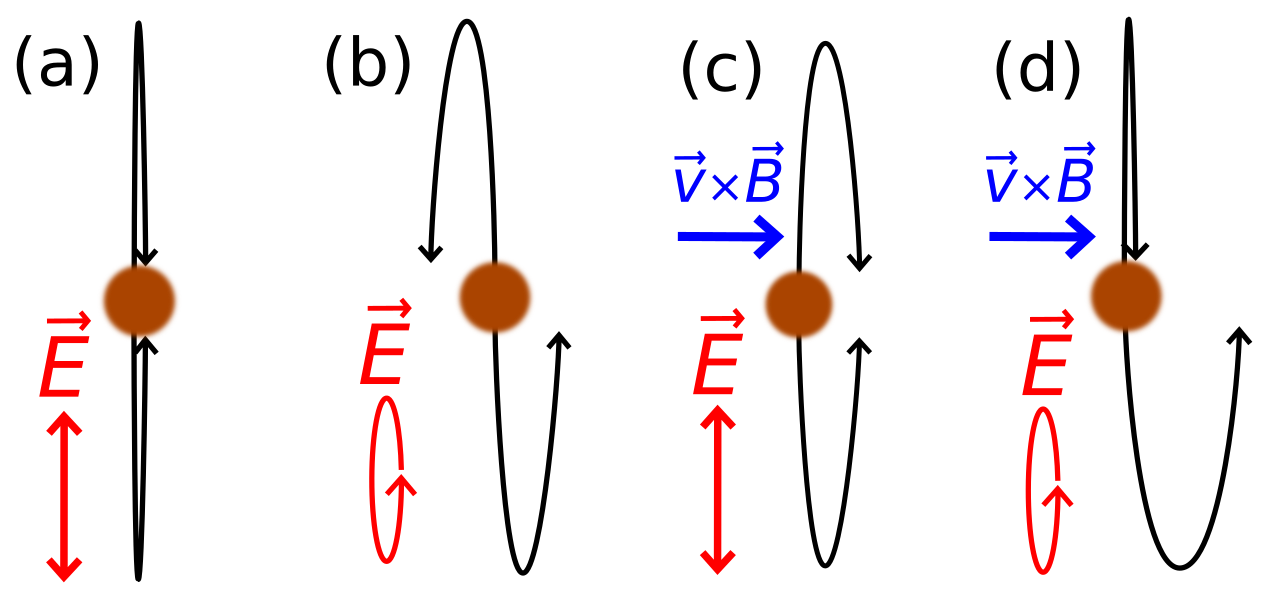
\includegraphics[width=0.55\textwidth]{9-Nondipole-HHG/Figures/figure9C.png} 
  \caption[
  Schematic electron trajectories in a forwards-elliptical field, with the effect of the ellipticity, the Lorentz force, and their combination
  ]{
  Schematic trajectories for the beam configuration of \reffig{f8-field-configuration}. The usual linear trajectories~\protect\subref{f8-schematic-trajectories-a} are shifted by the ellipticity~\protect\subref{f8-schematic-trajectories-b}, which cancels the Lorentz drift that would otherwise occur for a linear driver~\protect\subref{f8-schematic-trajectories-c}, driving the electron back to the ion~\protect\subref{f8-schematic-trajectories-d} and thereby re-enabling the harmonic emission.
  }
\label{f8-schematic-trajectories}
\end{figure}



Moreover, because this even-harmonics signal depends on the \textit{difference} between the two radiation bursts, it can be measurable even if the Lorentz-force effect is small. This means, in turn, that the mechanism can be used to provide an experimental observation of the Lorentz-force effect within HHG: because it requires very high intensities and long wavelenths, the effect has only been observed in ionization experiments~\cite{smeenk_partitioning_2011, ludwig_breakdown_2014}, but its presence is yet to be confirmed within HHG, and the onset of the harmonic die-out shown in \reffig{f6-emelina-original-spectrum} is still technologically some way away. However, as we shall see, the even harmonics signal is strong enough to be detected by sources that are currently available.


Here it is interesting to remark that the even-harmonics signal, in fact, depends interferometrically on the difference between the two radiation bursts, so it can be triggered by a difference in phase as well as in amplitude. This radically changes the scaling of the signal with respect to the experimental parameters -- it goes linearly with the ratio of the Lorentz drift to the wavepacket width, instead of quadratically, making it much easier to detect. In this chapter we will not explicitly trace the even-harmonics signal to the difference in phase between the two radiation bursts (as opposed to a difference in amplitude), leaving that for future work, but the calculated strength of the even harmonics is sufficient for the experimental prediction, and strong evidence that interferometric effects are indeed present.




It is also important to note the strong connections of this experiment to the bicircular experiments described in chapter~\ref{chap:spin-HHG}. Here, as opposed to the collinear, bichromatic experiments described there, we have single-frequency fields in a non-collinear arrangement, but much of the spirit of the results there holds: the selection rules are still valid, and in the photon picture each harmonic photon comes from $n$ photons from one beam and $n\pm1$ photons from the other, except that now the effect of this selection rule is not in energy but in the transverse momentum of the photon. Thus, each harmonic is confined to two symmetric spots on either side of the centreline. This has, in fact, been observed experimentally by D.\,Hickstein and co-workers~\cite{hickstein_non-collinear_2015}, and we refer the reader there for a closer analysis of the angular selection rules.


Similarly, and as we argued in section~\ref{sec:hhg-selection-rules}, this photon picture is grounded in the symmetries of the experiment. In this specific case, the two counter-rotating beams set up a polarization grating across the focus, as shown in \reffig{f8-field-configuration-ellipses}, with the direction of the main polarization rotating as the phase between the two beams changes across the focus. In this chapter, however, we will ignore the effects of this polarization grating, concentrating on the microscopic emission from a single location where the forwards ellipticity is strongest. 

Likewise, we will leave for future work the photon-picture and far-field propagation properties of the even harmonics, focusing only on their strength at the place where their emission is maximal. While this leaves open the question of how strong the overall even-harmonics emission will be, it also leaves untouched another major advantage of the even-harmonics signal -- that the even harmonics must, by symmetry, be spatially separated from the odd-harmonics signal, making their detection far easier.



The possibility of a forwards-elliptical field, with its polarization ellipse along the propagation direction, runs counter to most of the intuitions built by standard plane-wave vacuum electrodynamics, but it is indeed possible. Moreover, this configuration provides a flexible, readily available experimental setup, especially when compared to the challenging experimental proposals we considered earlier. 

In particular, the non-collinear beams allow the focal spot size (and therefore the laser intensity) to be decoupled from the degree of forwards ellipticity. This ability is crucial, since it allows the ionization fraction to be tuned for phase-matching, and more generally (and in contrast to the tight-focusing scheme of Refs.~\citealp{galloway_lorentz_2016} and \citealp{lin_tight-focus_2006}) it makes the entire focal geometry available as a tool for phase matching. This then makes the scheme light and flexible, with a lot of scope to adapt to multiple different requirements.




\section{High-order harmonic generation beyond the dipole approximation}

To bring things on a more concrete footing, we consider the harmonics generated in a noble gas by two beams with opposite circular polarizations propagating in the $x,z$ plane (in the reference frame of \reffig{f8-field-configuration-beams}), with wavevectors 
\begin{equation}
\mathbf k_\pm=k(\pm \sin(\theta),0,\cos(\theta)),
\end{equation}
where the angle $\theta$ to the centreline on the $z$ axis is typically small. The vector potential therefore reads
\begin{align}
\vba  (\vbr,t)
& =
\sum_\pm
\frac{F}{2\omega}
\begin{pmatrix}
\cos(\theta)\cos(\vbk_\pm\cdot\vbr-\omega t) \\
\pm\sin(\vbk_\pm\cdot\vbr-\omega t)\\
\pm\sin(\theta)\cos(\vbk_\pm\cdot\vbr-\omega t)
\end{pmatrix}
\nonumber \\ & =
\frac{F}{\omega}
\begin{pmatrix}
\phantom{-}  \cos(\theta)\cos(kz\cos(\theta)-\omega t)\cos(kx\sin(\theta)) \\
\phantom{-\sin(\theta)}  \cos(kz\cos(\theta)-\omega t)\sin(kx\sin(\theta))\\
-\sin(\theta)\sin(kz\cos(\theta)-\omega t)\sin(kx\sin(\theta))
\end{pmatrix}.
\label{e9-full-field}
\end{align}



As an initial approximation, for small $\theta$, the polarization planes coincide, and the polarization becomes linear, with a direction which rotates across the focus: 
\begin{equation}
\vba(\vbr,t)
\approx
\frac{F}{\omega}
\begin{pmatrix}
\cos(kx\sin(\theta)) \\
\sin(kx\sin(\theta)) \\
0
\end{pmatrix}
\cos(\omega t),
\end{equation}
where we set $z=0$ and therefore just examine a single transverse plane. However, when taken in full, the vector potential has a slight ellipticity, with a maximal value of $\eps = \sin(\theta)$ when $kx\sin(\theta)=\tfrac{\pi}{2}$, in which case
\begin{equation}
\vba  (\vbr,t)
=
\frac{F}{\omega}
\begin{pmatrix}
0 \\
\:\:\cos(\omega t)\\
\sin(\theta)\sin(\omega t)
\end{pmatrix}.
\label{e9-forwards-elliptical-field}
\end{equation}



In experiments, the beam half-angle $\theta$ will typically be small, on the order of \SI{1}{\degree} to~\SI{51}{\degree}~\cite{hickstein_non-collinear_2015}, with corresponding ellipticities of up to $\eps=\sin(\theta)\approx 9\%$, which is enough to counteract even significant magnetic drifts while still maintaining a flexible experimental scheme. 

The generation of harmonics beyond the breakdown of the dipole approximation has been described in a fully-relativistic treatment~\cite{milosevic_qm-sfa-ultrahigh-hhg_2000, milosevic_relativistic_2002, milosevic_relativistic_2002-1}, but this can be relaxed to the usual Strong-Field Approximation, as we  developed it in section~\ref{sec:lewenstein-hhg}, with appropriate modifications to include non-dipole effects~\cite{ walser_hhg_2000, kylstra_photon_2001, kylstra_photon_2002, chirila_nondipole_2002, chirila_analysis_2004}. (Similarly, full TDSE simulations are possible~\cite{ meharg_beyond-dipole-tdse_2005}, but they become very demanding in this regime.)


If a single beam is present, non-dipole terms break the dipole selection rules and produce even harmonics, but these are polarized along the propagation direction and therefore do not propagate on axis. The use of multiple beams in the non-dipole regime allows for observable breakdowns of the selection rules~\cite{averbukh_stability_2002}, and indeed the generation of harmonics in this beyond-dipole regime has been explored for multiple-beam configurations by V.\,Averbukh and co-workers in \citer{averbukh_stability_2002}, but the available results are only valid for very restricted beam arrangements. In the rest of this section, then, we will extend the available formalism, pioneered by N.\,J.\,Kylstra and co-workers~\cite{kylstra_photon_2001, kylstra_photon_2002, chirila_nondipole_2002, chirila_analysis_2004} to arbitrary beam configurations.




As we noted earlier, the presence of the Lorentz force as a factor in high-order harmonic generation represents the breakdown in the dipole approximation, for the simple reason that in the dipole approximation there is no magnetic field present. Or, to put this another way, ignoring the spatial variation of the vector potential also completely zeroes out its curl, and therefore the magnetic field. Conversely, if we want to describe the effect of the magnetic field, then we need to go beyond the dipole approximation and include the spatial variation of the vector potential. For our purposes, however, it is sufficient to consider this to first order 








We start, therefore, with the Coulomb-gauge hamiltonian, with the spatial variation of $\mathbf A$ taken to first order in $\mathbf r$,
\begin{align}
\hat H_V & = \frac 12\left(\hat \vbp+\vba(\hat \vbr,t)\right)^2+\hat V_0
 \\ & = \frac 12\left(\hat \vbp+\vba(\vb 0,t)+(\hat \vbr\cdot\nabla)\vba(\vb0,t)\right)^2+\hat V_0.
\end{align}
We then perform a unitary transformation to $\ket{\Psi_L}=e^{i\hat \vbr\cdot \vba(\vb0,t)} \ket{\Psi_V}$, as in the dipole case, and we define this as the length gauge. Here the hamiltonian reads
\begin{equation}
\hat H_L = \frac 12\left(\hat \vbp+(\hat \vbr\cdot\nabla)\vba(\vb0,t)\right)^2+\hat \vbr\cdot\vbf(t)+\hat V_0,
\end{equation}
with $\vbf(t)=-\tfrac{\partial\vba}{\partial t}(\vb0,t)$. Moreover, we neglect terms in $\left((\hat \vbr\cdot\nabla)\vba(\vb0,t)\right)^2$ for consistency, 
as they are of higher order in $kr$, to get our final hamiltonian
\begin{equation}
H_L = \frac{\hat{\vbp}^2}{2} + \hat \vbr\cdot\vbf(t) + \hat\vbr\cdot\gradA(t)\cdot\hat\vbp + \hat V_0
 = \hat H_\mathrm{las}+\hat V_0.
\label{e9-length-gauge-hamiltonian}
\end{equation}
Here the gradient $\gradA(t)$ denotes a matrix whose $i,j$-th entry is $\frac{\partial A_j}{\partial x_i}(\vb0,t)$, so in 
component notation the laser-only hamiltonian reads
\begin{equation}
\hat H_\mathrm{las} = \frac{\hat\vbp^2 \!\! }{2}+\hat x_jF_j(t)+\hat x_j\frac{\partial A_k}{\partial x_j}(t)\hat p_k,
\label{e9-laser-only-hamiltonian}
\end{equation}
with summations over repeated indices understood.%
\footnote{%
As an anonymous referee pointed out, the hamiltonian in equations \eqref{e9-length-gauge-hamiltonian} and \eqref{e9-laser-only-hamiltonian} is not obviously hermitian at an initial glance. However, it is quite easy to see that the order of $\hat x_j$ and $\hat p_k$ does not affect the hamiltonian, since the difference between the two orderings reduces to the commutator $[x_j,p_k]$, via
$$
\hat x_j\frac{\partial A_k}{\partial x_j}(t)\hat p_k - \hat p_k\frac{\partial A_k}{\partial x_j}(t)\hat x_j
= \left[ \hat x_j , \hat p_k\right] \frac{\partial A_k}{\partial x_j}(t)
=i\hbar\delta_{jk} \frac{\partial A_k}{\partial x_j}(t) 
= i \hbar \frac{\partial A_k}{\partial x_k}(t) 
= i\hbar \nabla \!\cdot\! \vba(\vb0,t) = 0.$$
The difference therefore comes down to the divergence of the vector potential (as, indeed, it does for the more general term $\vba(\vbr,t)\cdot\vbp$ of the standard coupling), and this vanishes in the radiation gauge. This is, of course, rather standard material~\cite{cohen-tannoudji_photons-and-atoms}.
}




Calculating the harmonic emission caused by the hamiltonian \eqref{e9-length-gauge-hamiltonian} is essentially as simple as in the dipole case, and one only needs to modify the continuum wavefunction to include the non-dipole term. We are looking, then, for non-dipole, non-relativistic Volkov states, which should obey the Schrödinger equation for the laser-only hamiltonian $\hat H_\mathrm{las}$,
\begin{equation}
i\frac{\d}{\d t}\volkov{\vbp}{t} = \hat H_\mathrm{las}(t) \volkov{\vbp}{t} 
\end{equation}
and which remain eigenstates of the momentum operator throughout. 


To generalize the dipole Volkov states, which we know from \eqref{e2-volkov-wavefunctions}, we begin by phrasing them in the form
\begin{equation}
\volkov{\vbp}{t}=e^{-\frac i2 \int^t\vbpi(\vbp,\tau)^2\d \tau}\ket{\vbpi(\vbp,t)},
\label{e9-volkov-state-definition}
\end{equation}
where $\ket{\vbpi(\vbp,t)}$ is a plane wave at the kinematic momentum $\vbpi(\vbp,t)=\vbp+\vba(t)$, and then looking for appropriate modifications to $\vbpi(\vbp,t)$. 


Here, because of the requirement that the states remain eigenstates of the momentum operator throughout, we can in fact forget about the Volkov phase $e^{-\frac i2 \int^t\vbpi(\vbp,\tau)^2\d \tau}$ and simply look to generalize the time dependence of the spatial component, the shifting plane wave $\ket{\vbpi(\vbp,t)}$, which in the dipole case obeys the Schrödinger equation
\begin{equation}
i\frac{\d}{\d t}\ket{\vbpi(\vbp,t)} 
= 
\hat \vbr\cdot\vbf(t) \ket{\vbpi(\vbp,t)}.
\end{equation}


Similarly, for the nondipole case we include here the first-order variation of the potential, so we're looking for a solution of the Schrödinger equation
\begin{equation}
i\frac{\d}{\d t}\ket{\vbpi(\vbp,t)} 
= 
\left[\vphantom{\sum} \hat \vbr\cdot\vbf(t) + \hat\vbr\cdot\gradA(t)\cdot\hat\vbp \right]
\ket{\vbpi(\vbp,t)}.
\end{equation}
This equation is most easily solved by going briefly to the position representation, where we can obtain the time derivative
\begin{equation}
i\frac{\d}{\d t} \braket{\vbr}{\vbpi(\vbp,t)} 
=
i\frac{\d}{\d t} \frac{e^{i\vbr \cdot \vbpi(\vbp,t)}}{(2\pi)^{3/2}}
=
-\vbr \cdot \frac{\partial\vbpi(\vbp,t)}{\partial t}\frac{e^{i\vbr \cdot \vbpi(\vbp,t)}}{(2\pi)^{3/2}}
=
-\vbr \cdot \frac{\partial\vbpi(\vbp,t)}{\partial t} \braket{\vbr}{\vbpi(\vbp,t)}
,
\end{equation}
from which it follows that
\begin{equation}
i\frac{\d}{\d t} \ket{\vbpi(\vbp,t)} 
=
-\hat \vbr \cdot \frac{\partial\vbpi(\vbp,t)}{\partial t} \ket{\vbpi(\vbp,t)}
.
\end{equation}
Then, by setting $\hat\vbp \ket{\vbpi(\vbp,t)} = \vbpi(\vbp,t) \ket{\vbpi(\vbp,t)}$, the Schrödinger equation reduces to 
\begin{equation}
\hat \vbr\cdot \left[
 \vphantom{\sum} 
 \frac{\partial\vbpi(\vbp,t)}{\partial t}
 + \vbf(t) 
 + \gradA(t)\cdot \vbpi(\vbp,t)
\right]
\ket{\vbpi(\vbp,t)}
=0
,
\end{equation}
and from there to a simple equation for the kinematic momentum,
\begin{equation}
\frac{\partial\vbpi(\vbp,t)}{\partial t}
- \frac{\d \vba(t)}{\d t}
=
-\gradA(t)\cdot \vbpi(\vbp,t)
,
\label{e9-vbpi-evolution-equation}
\end{equation}
with the electric field $\vbf$ substituted as the time derivative of the vector potential.


The time evolution equation \eqref{e9-vbpi-evolution-equation} for $\vbpi(\vbp,t)$ is, formally speaking, an inhomogeneous time-dependent Schrödinger equation in three dimensions,  so it has a formal solution, via a time-ordered exponential of $\int \gradA(t)\:\d t$, but this is far too complex for our purposes. Since we're only looking for the first perturbation with respect to the nondipole terms, we can simply look for solutions around the dipole trajectory, $\vbpi( \vbp,t) =\vbp+\vba(t)$, and ask for the effect of the nondipole perturbation $-\gradA(t)\cdot \vbpi(\vbp,t)$.

%This means that we can simply perform a perturbative expansion for $\vbpi(\vbp,t)$,

To get this, we write $\vbpi(\vbp,t) = \vbp + \vba(t) +\vbpi^{(1)}(\vbp,t)$, in terms of the perturbation $\vbpi^{(1)}(\vbp,t)$, which obeys the equation
\begin{equation}
\frac{\partial\vbpi^{(1)}}{\partial t}(\vbp,t)
=
-\gradA(t)\cdot \left(\vbp + \vba(t) \right)
-\gradA(t)\cdot \vbpi^{(1)}(\vbp,t)
.
\end{equation}
Here we ignore the second term, $\gradA(t)\cdot \vbpi^{(1)}(\vbp,t)$, in the perturbative ethos. Alternatively, we leave it for a second-order correction if necessary, but since each time integral of the gradient introduces a factor of $\int\gradA\d\tau \sim \frac{k}{\omega}A= \frac{1}{c}A$, and our hamiltonian is only accurate to first order in $1/c$, then for consistency here we should drop the final term, reducing the equation to simply $\frac{\partial\vbpi^{(1)}}{\partial t}(\vbp,t) = -\gradA(t)\cdot \left(\vbp + \vba(t) \right)$, which can easily be solved to give
\begin{equation}
\vbpi(\vbp,t)=\vbp+\vba(t)-\int^t\gradA(\tau) \cdot (\vbp+\vba(\tau))\d\tau,
\label{e9-kinematic-momentum-nondipole}
\end{equation}
in terms of an indefinite integral $\int^t\d t$ of the right-hand side of \eqref{e9-vbpi-evolution-equation}. 


We have, then, our result -- the kinematic momentum of \eqref{e9-kinematic-momentum-nondipole}\,-- and this directly determines our nondipole nonrelativistic Volkov states via the same connection, \eqref{e9-volkov-state-definition}, as with the usual dipole Volkov wavefunctions. Since our modified Volkov states are (approximate) solutions of the continuum Schrödinger equation, they also yield directly a continuum propagator exactly as in \eqref{e7-volkov-propagator}. This means that we can just plug our nondipole continuum dynamics directly into the rest of the SFA calculation of the HHG amplitude. Then it is straightforward to take this directly to the harmonic dipole, which comes out in the form
\begin{equation}
\vb D(t)
=
\int_{-\infty}^t \!\!\d t'\!
\int\!\d\vbp\:
\vbd(\vbpi(\vbp,t))
e^{iS(\vbp,t,t')}
\vbf(t')\cdot\vbd(\vbpi(\vbp,t'))
+\cc
\label{e9-initial-harmonic-dipole}
\end{equation}
Here the action also retains its essential form as
\begin{equation}
S(\vbp,t,t')=I_p(t-t')+\frac12 \int_{t'}^t \vbpi(\vbp,\tau)^2\d\tau
,
\label{e9-initial-action}
\end{equation}
with the only change coming in the kinematic momentum $\vbpi(\vbp,t)$, which is now given by~\eqref{e9-kinematic-momentum-nondipole}. This result is a generalization to an arbitrary monochromatic vector potential of the results of Refs.~\citealp{ kylstra_photon_2001, kylstra_photon_2002, chirila_analysis_2004, chirila_nondipole_2002}, and it is consistent with those results when restricted to their single-beam settings.



However, the above formalism is not quite sufficient in the presence of multiple beams, because it turns out that the antiderivative 
\begin{equation}
\int^t\gradA(\tau) \cdot \vba(\tau)\d\tau,
\label{e9-trouble-integral}
\end{equation}
from \eqref{e9-kinematic-momentum-nondipole}, can no longer be uniquely defined. In general, this occurs in the presence of multiple beams at nontrivial angles and with nontrivial phases, but when that happens the cross terms in $\gradA(\tau) \cdot \vba(\tau)$ are oscillatory about a nonzero average. This then causes the integral~\eqref{e9-trouble-integral} to contain a linearly-increasing term, whose constant of integration is harder to pin down than the usual oscillatory terms.

Here it bears explaining that in the previous work on the subject~\cite{kylstra_photon_2001, kylstra_photon_2002, chirila_analysis_2004, chirila_nondipole_2002}, this problem was not present, because if one only considers a monochromatic field of the form $\A(\vbr,t)=A_0\ue \cos(\vbk\cdot \vbr -\omega t)$, then the integrand in \eqref{e9-trouble-integral} can be explicitly calculated, giving
\begin{align}
\gradA(t) \cdot \vba(t) 
=
\gradA(\vb0,t) \cdot \vba(\vb0,t) 
=  
\vbk A_0^2 \sin(\omega t)\cos(\omega t)
.
\end{align}
This oscillates about an average of zero, because the phase shift  between $\vba(t)$ and its spatial derivative is precisely \SI{90}{\degree}. This then implies that for the problem to come up one needs to consider multiple beams, for which the cross terms in \eqref{e9-trouble-integral} can oscillate about a nonzero average; interestingly, the only multi-beam paper in this formalism, \citer{averbukh_stability_2002}, only deals with beam configurations with orthogonal polarizations, for which the inner product of \eqref{e9-trouble-integral} also zeroes out the problem. 

In previous work, then, the indefinite integral of \eqref{e9-kinematic-momentum-nondipole} has only appeared with oscillatory trigonometric functions inside it, and these can be unambiguously assigned a preferred antiderivative by replacing cosines with sines and sines with (minus) cosines. For a general monochromatic field, however, this is no longer the case, and the integral in \eqref{e9-trouble-integral} can have a constant term in the integrand, which causes our kinematic momentum $\vbpi(\vbp,t)$ to have a linearly-increasing term.



This effect, in fact, is real and physical, going beyond our specific mathematics, and it reflects the fact that the kinematic momentum is indeed subject to a linear walk-off: that is, a constant force in the $x,y$ plane, orthogonal to the laser propagation direction $z$, in addition to the usual oscillations; we show this in \reffig{f9-trajectory}. This constant force results from the interplay between the magnetic field and the $z$-direction velocity imparted by the elliptical electric field.



\begin{figure}[htb]
  \centering
  
  \subfloat{\label{f9-trajectory-xz}}
  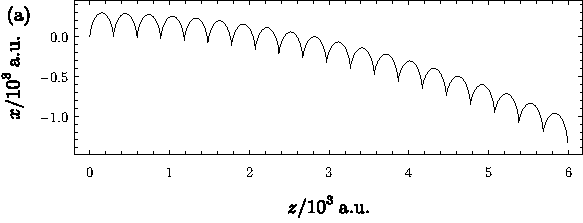
\includegraphics[scale=1]{9-Nondipole-HHG/Figures/figure9Da.pdf}
  \hspace{9mm}$\,$
  
  \vspace{5mm}
  
  \subfloat{\label{f9-trajectory-yz}}
  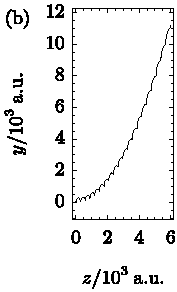
\includegraphics[scale=1]{9-Nondipole-HHG/Figures/figure9Db.pdf} 
  \hspace{5mm}
  \subfloat{\label{f9-trajectory-3d}}
  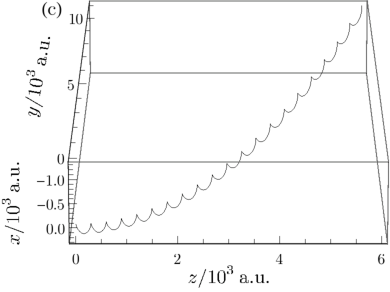
\includegraphics[scale=1]{9-Nondipole-HHG/Figures/figure9Dc.pdf} 
  
  \captionsetup{width=\textwidth}
  \caption[
  Classical trajectory of a particle released at the peak of the field in two noncollinear bicircular fields, showing transverse acceleration across the focus
  ]{
  The classical trajectory of a particle released at rest at the peak of the field from~\eqref{e9-full-field} exhibits oscillations about a central position which accelerates uniformly transversely across the focus, with a parabolic trajectory. The effect is generally slight, and the parameters here (\SI{1.6}{\micro\meter} beams at $\SI{e15}{W/cm^2}$ with $\theta=\SI{20}{\degree}$ at $kx\sin(\theta)=\SI{15}{\degree}$) are somewhat exaggerated, but the loss of periodicity in \eqref{e9-initial-harmonic-dipole} is serious. Similarly, the effect is only visually apparent over multiple oscillations, but even on the first oscillation the effect changes the time of recollision and therefore has a strong effect on the harmonic emission. This effect is also present for drivers with linear polarization in the common plane of propagation.
  }
\label{f9-trajectory}
\end{figure}


In practical terms, the effect is small, but even in the first period it affects the timing of the ionization and recollision events, so it has a strong effect on the harmonic emission. As such, if it is not handled correctly then it can introduce noise in a numerically calculated spectrum (especially for monochromatic fields with no edge clipping, where aperiodicities in the signal have a large effect) at the same level as the non-dipole signal we are looking to detect, thereby ruining the spectrum.




From a more mathematical perspective, this effect implies that states given by \eqref{e9-volkov-state-definition} and \eqref{e9-kinematic-momentum-nondipole} cease to be Floquet states of the laser hamiltonian when the dipole approximation breaks down. The Floquet states in this case are known in terms of Airy functions~\cite{Li-Reichl-Floquet} but those solutions are not very useful in this context. The nondipole Volkov states we use still form a basis of (approximate) solutions of the Schrödinger equation, but now they require an initial condition.




To choose the appropriate initial condition, we note that the linear walk-off represents a secular term~\cite{Nayfeh_secular_terms} in these solutions, and we minimize the effect of this secular term by choosing an explicit reference time at the moment of ionization:
\begin{equation}
\vbpi(\vbp,t,t')=\vbp+\vba(t)-\int_{t'}^t \gradA(\tau) \cdot (\vbp+\vba(\tau))\d\tau.
\label{e9-modified-kinematic-momentum-nondipole}
\end{equation}
This then trickles down to the action,
\begin{equation}
S(\vbp,t,t')=I_p(t-t')+\frac12 \int_{t'}^t \vbpi(\vbp,\tau,t')^2\d\tau,
\label{e9-modified-action}
\end{equation}
and to the harmonic dipole
\begin{align}
\vb D(t)
=
\int_{-\infty}^t \!\!\d t'\!
\int\!\d\vbp\:
&
\vbd(\vbpi(\vbp,t,t'))
e^{iS(\vbp,t,t')}
%\nonumber \\ & \quad
\times\vbf(t')\cdot\vbd(\vbpi(\vbp,t',t'))
+\cc
\label{e9-modified-harmonic-dipole}
\end{align}
by going through the same steps as in section~\ref{sec:lewenstein-hhg} once again.
 
This harmonic dipole is sufficient to evaluate the harmonic emission from arbitrary beam configurations, and it can be further simplified by the use of the saddle-point approximation for the momentum integral and, if required, the Uniform Approximation~\cite{figueira_uniform-approximation_2002, milosevic_long-quantum-orbits_2002} for the temporal integrals. Our implementation, based on \eqref{e9-modified-harmonic-dipole}, is available from~\citer{RB-SFA}.









\section{Results}

We have, then, a suitable tool for calculating the harmonics emitted by this system, so we turn now to the resultant spectra. Here we concentrate on the single-atom emission at the point of maximal forwards ellipticity, though of course the tool is ready for further use on the problem, and this will be the focus of future work.




There are two main avenues of interest in our results: the recovery of harmonic emission from the Lorentz-drift-induced dropdown in the deep nondipole regime, where the harmonic yield would otherwise essentially disappear, as in \reffig{f6-emelina-original-spectrum}, and the emission of even harmonics in the moderately non-dipolar regime, which is accessible to current sources.



\begin{figure}[p]
  \centering
  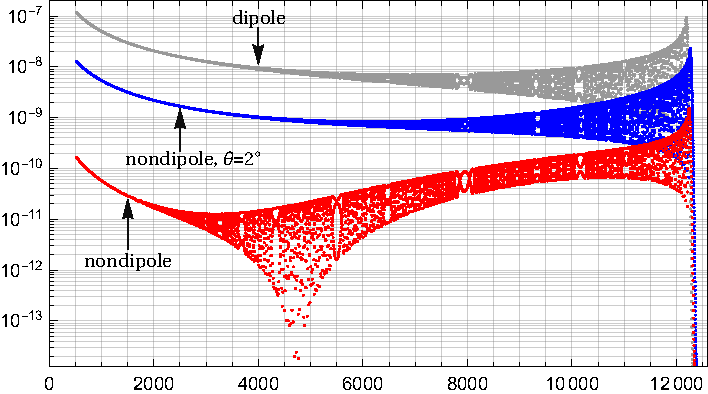
\includegraphics[width=0.65\textwidth]{9-Nondipole-HHG/Figures/figure9F.pdf} 
  \caption[
  Harmonic emission from a Ne$^{6+}$ ion in an $\SI{800}{nm}$ field of intensity $I=\SI{e17}{W/cm^2}$, showing the damping from nondipole effects and the recovery when the beams are non-collinear
  ]{
  Above-threshold harmonic emission for a Ne$^{6+}$ ion in an $\SI{800}{nm}$ field of intensity $I=\SI{e17}{W/cm^2}$, calculated in the uniform approximation using the first pair of quantum orbits, and discarding $z$-polarized harmonics. For linear polarization, the dipole-approximation emission drops by two orders of magnitude when nondipole effects are included, but adding in even a small forwards ellipticity at $\theta=2\si{\degree}$ can help recover the harmonic emission. 
  }
\label{f8-harmonic-recovery-spectra}
\end{figure}


\newlength{\figureNineEheight}
\setlength{\figureNineEheight}{4.2cm}
{
\setlength\tabcolsep{0mm}
\begin{figure}[p]
  \centering
  \scriptsize
  \begin{tabular}{ccc}
    & (a) \SI{800}{nm}, \SI{3.2e14}{W/cm^2}
    & (b) \SI{800}{nm}, \SI{e15}{W/cm^2}
    \\
    \rotatebox{90}{\hspace{9mm} $|\omega^2\widetilde{\vbD}(\omega)|^2$ (arb.\,u.)}
    \vspace{2mm}
    &
 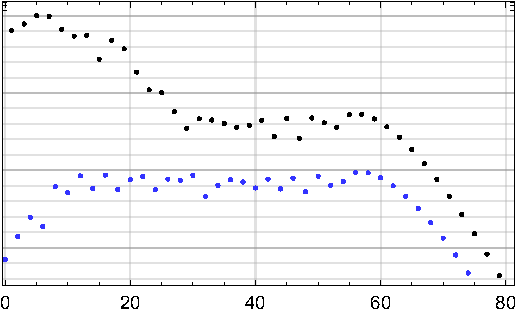
\includegraphics[height=\figureNineEheight]{9-Nondipole-HHG/Figures/figure9Ea.pdf}
    & 
 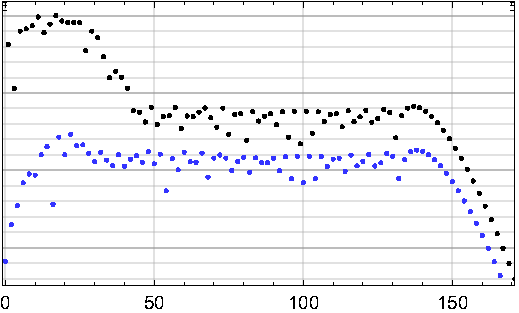
\includegraphics[height=\figureNineEheight]{9-Nondipole-HHG/Figures/figure9Eb.pdf}
   \\[4mm]
    & (c) \SI{1.6}{\micro\metre}, \SI{3.2e14}{W/cm^2}
    & (d) \SI{1.6}{\micro\metre}, \SI{e15}{W/cm^2}
    \\
    \rotatebox{90}{\hspace{9mm} $|\omega^2\widetilde{\vbD}(\omega)|^2$ (arb.\,u.)}
    \vspace{2mm}
    &
 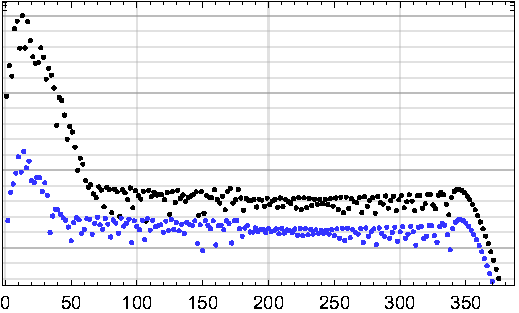
\includegraphics[height=\figureNineEheight]{9-Nondipole-HHG/Figures/figure9Ec.pdf}
    & 
 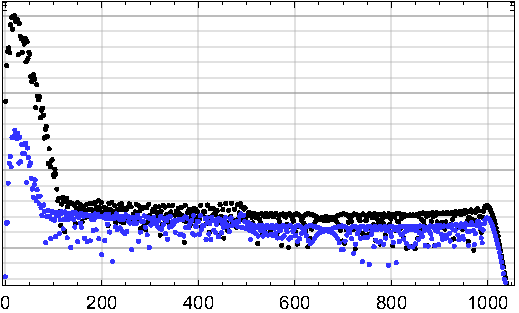
\includegraphics[height=\figureNineEheight]{9-Nondipole-HHG/Figures/figure9Ed.pdf}
   \\[2mm]
    & harmonic order & harmonic order 
  \end{tabular}
  \caption[
  Harmonic spectra for reasonable fields at $\SI{800}{nm}$ and $\SI{1.6}{\micro\metre}$, and intensities $3.2\times 10^{14}$ and $\SI{e15}{W/cm^2}$, showing measurable even-harmonics signals for non-collinear beams
  ]{
  Harmonic spectra ($\bullet$ odd and {\color{blue!80}$\bullet$} even harmonics) produced in helium in the non-dipole regime for intensities of $3.2\times 10^{14}$ and $\SI{e15}{W/cm^2}$ and monochromatic fields of \SI{800}{nm} and \SI{1.6}{\micro\metre} at a beam half-angle of $\theta=4\si{\degree}$, on arbitrary scales and eliminating $z$-polarized harmonics. The intensity ratio between even and odd harmonics varies from ${\sim}10^{-3}$ for \SI{800}{nm} drivers to ${\sim}10\%$ for strong mid-IR fields at $\SI{1.6}{\micro\metre}$ and $\SI{e15}{W/cm^2}$. The required sources are on the high end of intensity at the given wavelengths, but they are already accessible with current technology.
  }
\label{f9-even-harmonics-spectra}
\end{figure}
}


To showcase the former, we present in \reffig{f8-harmonic-recovery-spectra} the harmonic emission of a highly charged neon ion in a very intense $\SI{800}{nm}$ field.%
%
\footnote{%
Ideally, this should be done for a field of more moderate intensity by taking a longer wavelength, as in the calculation of \citer{emelina_possibility_2014} shown in \reffig{f8-harmonic-recovery-spectra}. The choice to use the high-intensity, moderate-wavelength regime in \reffig{f8-harmonic-recovery-spectra} is to reduce the computational load on this initial application: at equal harmonic cutoff, a smaller photon energy requires the calculation of more harmonics. However, since both directions are in the deep $\gamma\ll1$ regime, the nondipole SFA dynamics are essentially equivalent.
}
%
(These conditions are essentially equivalent to Fig.~2b of \cite{ chirila_nondipole_2002}, though in \reffig{f8-harmonic-recovery-spectra} we keep only the first pair of quantum orbits for~clarity.)
It is easy to see that the `ideal' harmonic yield, given by the standard Lewenstein SFA in the dipole approximation, drops down significantly once nondipole terms are introduced (and, indeed, it continues to drop if the intensity is increased). However, introducing even a small forwards ellipticity, with only a $\theta=\SI{2}{\degree}$ half-angle between the non-collinear bicircular beams, can do much to restore the harmonic~emission.

Here it is also important to note that these results have only been very partially optimized, and that the harmonic recovery can certainly work better than displayed here. Moreover, the curves as shown are slightly misleading: the blue curve, showing the recovered nondipole harmonics, contains both even and odd harmonics in essentially equal measure (as can be seen e.g. in the under-resolved quantum-path-interference feature near harmonic order 8000), so its spectral energy density should be considered to be twice the~shown yield. 

Similarly, the `ideal' curve to compare to is not exactly the full dipole-approximation yield, since that contains two recollisions per half cycle, but as we discussed in \reffig{f8-schematic-trajectories} we can only hope to recover one of the two recollisions. Thus, we should consider the target intensity to be half of the shown dipole-approximation yield, which means that the gap as displayed, between the recovered nondipole emission in blue and the target dipole-approximation emission in gray, is exaggerated by a factor of four. Once this is taken into account, the shown spectrum recovers essentially all of the signal at cutoff, and it is only down by a factor of two from the target over most of the spectrum.


On the other hand, it is a curious observation that the cutoff has been extended slightly in the recovered emission. This is almost definitely an artefact of the method, chiefly of the non-relativistic approximation, since the cutoff in fully relativistic SFA calculations has been shown to decrease noticeably~\cite{milosevic_relativistic_2002-1}. Planned calculations using a fully relativistic theory should remove this artefact, but they are extremely unlikely to change the overall enhancement, since the basic physics is preserved.



In addition to this, there are also important results on the generation of even harmonics by more moderate fields, which we present in \reffig{f9-even-harmonics-spectra} for helium in the non-dipole regime at intensities of $3.2\times 10^{14}$ and $\SI{e15}{W/cm^2}$ and for driver wavelengths of $\SI{800}{nm}$ and $\SI{1.6}{\micro\metre}$. It should be noted that the non-dipole even harmonics approach detectable intensities, between 0.1\% and 1\% of the energy of the odd harmonics, even for $\SI{800}{nm}$ drivers at the relatively reasonable intensity of $\SI{e15}{W/cm^2}$, which is easily accessible to modern titanium-sapphire laser systems.


Similarly, when the wavelength is increased to $\SI{1.6}{\micro\metre}$, at a maximum intensity of $\SI{e15}{W/cm^2}$ that is within the range of current optical parametric chirped-pulse amplifiers, the contrast ratio between the even and odd harmonics increases even further, reaching into the 10\% of energy in the even harmonics, which is certainly measurable using current detectors.



In addition to this, the even harmonics should also be angularly separated from the dipole-allowed odd harmonics. This angular separation results from the conservation of momentum, and it was clearly demonstrated for the dipole harmonics by Hickstein \mbox{et al.}~\cite{hickstein_non-collinear_2015}: these must absorb an odd number of photons, but the conservation of spin angular momentum~\cite{fleischer_spin_2014, Pisanty_spin_conservation_2014} requires the harmonic to form from $n$ photons of one beam and $n+1$ photons from the other, resulting in a net transverse momentum of $\pm\hbar k_x = \pm\hbar k\sin(\theta)$ for the odd harmonics. The even harmonics represent the parametric conversion of an even number of photons, via the tensor operator $\hat{\vbr}\otimes\hat{\vbp} \mathbin{:} \nabla \hspace{-0.15em} \vba$, and they can therefore absorb either zero transversal momentum -- resulting in linear polarization along the $y$ axis -- or $\pm2\hbar k_x$, with opposite circular polarizations. These even harmonics, then, should appear at distinctly resolvable spots in the far field, which greatly simplifies their detection.

As a final note, it is important to remark that it is the interferometric quality of our scheme that enables the detection of nondipole effects, by unbalancing (both in phase and in amplitude) the interferometer which would otherwise suppress the even harmonics, and this changes the scaling of this behaviour. In general, the wavepacket displacement scales as
$d \propto {F^2}/{2c\omega^3}$,
and the wavepacket width goes as 
$\Delta x \propto {F^{1/2}}/{(2I_p)^{1/4}}$~\cite{hatsagortsyan_laser_driven_2008},
so the normalized displacement scales as 
\begin{equation}
\zeta=\frac{d}{\Delta x}\propto \frac{(2I_p)^{1/4}F^{3/2}}{2c\omega^3}.
\end{equation}
The strength of the even harmonics, which arises from an interferometric effect, is linear in $\zeta$, while the drift-induced reduction in harmonic emission follows the gaussian shape of the wavepacket and therefore scales with $\eta=\zeta^2=(d/\Delta x)^2$, which explains why the nondipole effects are still some way in the future in terms of detecting the drop-off in harmonic efficiency, but still easily observable with currently available sources in our results.









\section{Outlook}
In this chapter we built a flexible and powerful tool for calculating harmonic emissions, and we described the framework for a broad and varied subject matter in the experimental scheme we proposed, but we left several avenues unexplored, and these form clear avenues for future work.

Most importantly, the spatial variation of the polarization across the focus is a crucial ingredient of the dynamics, as is clear from the far-field dynamics observed in the existing, low-intensity experiment~\cite{hickstein_non-collinear_2015}, and these become richer once the forwards ellipticity is introduced and doubly so with nondipole effects, so it is certainly necessary to investigate the behaviour of the harmonics across the focus.

Similarly, on a more theoretical note, the photon-picture properties of the nondipole even harmonics still need a coherent picture; this is also relevant in the planning of experiments to detect those even harmonics, which require a good understanding of their propagation to the far field.

On another track, we showed that the even-harmonics signal is far stronger than would be expected for only an amplitude imbalance in the intra-cycle interferometer that, in the dipole case, rules out the even harmonics. However, there is still some work to be done to show that there is, in fact, a phase imbalance as well, and to quantify this phase imbalance in terms simple enough to be helpful in predicting features of the experiment. 

Likewise, the scaling properties of all of these harmonics bear further investigation, particularly so for the even harmonics. These should scale with $\zeta = d/\Delta x$, but this should still be confirmed with explicit SFA calculations, since knowledge of this scaling law is of essential importance to designing specific experiments that implement the scheme.

Going a bit further than this, it is also important to investigate in more detail the effect of phase matching on the features we investigated here and in the future work we propose, especially so for several features of the far-field spectrum that turn out to depend sensitively on changes in the intensity, and which require closer integration with propagation simulations to produce reliable experimental predictions.

On a somewhat broader scale, the tools we have built in this chapter are also directly applicable to the tight-focus and waveguide geometries~\cite{ galloway_lorentz_2016}, in which they should help uncover very rich spatial dynamics inside the focus, with the phase effects evidenced by the strong scaling of our even harmonics likely playing a leading role. Similarly, our beyond-dipole SFA is likely to be directly applicable to the generation of high-order harmonics in nanostructures, where the vector potential changes in length scale of the electron excursion~\cite{chacon_hhg-plasmonic_2015, ciappina_attosecond-nanoscale_2016}.

More generally, though, the generation of even harmonics from nondipole, Lorentz-force effect is an experiment, available to current technology, waiting to be implemented, and much of the interesting work ahead lies in the design and implementation of such an experiment.














































